%%%%%%%%%%%%%%%%%%%%%%%%%%%%%%%%%%%%%%%%%%%%%%%%%%%%%
%			HLAVIČKA								%
%%%%%%%%%%%%%%%%%%%%%%%%%%%%%%%%%%%%%%%%%%%%%%%%%%%%%
\documentclass[openany,12pt]{memoir}

\usepackage[utf8]{inputenc} 
\usepackage[czech]{babel}
\usepackage[T1]{fontenc}
\usepackage[top=1.5cm, bottom=2cm, left=2cm, right=2cm]{geometry}  % --> NASTAVENÍ OKRAJŮ
\usepackage{fancyhdr}
\usepackage{graphicx}
%\usepackage{lmodern}
\usepackage{tgschola}  % --- Silnější font
\usepackage{xwatermark}
\usepackage{xcolor}
\usepackage{changepage}
\usepackage{newunicodechar}



%%%%%% Package na zpěvník
\usepackage[full]{leadsheets}%http://mirrors.nic.cz/tex-archive/macros/latex/contrib/leadsheets/leadsheets_en.pdf   --> dokumentace	
\definesongtitletemplate{empty}{} 
\setchords{
format = \bfseries,   %tučné akordy
minor = {mi},% 
input-notation = {german},%
output-notation = {german}%
}
\definesongtitletemplate{empty}{} 

\newlength{\drop}
\newwatermark[allpages,color=red!50,angle=0,scale=2, xpos=0,ypos=0]{
\includegraphics[width=5cm]{obr/pozadi2.jpg}} %--> dvojka na pozadí


%%%% Vlastní příkazy
\newcounter{Slokočet}   %Automatické číslování slok
\newcommand{\mezera}{\vspace*{0.5cm}}   %Horizontální odsazení slok
\newcommand{\stred}{5.2cm}   %%% Na zarovnání slok doprostřed, pozn. automatičtější zarovnávání na střed nejde
\newcommand{\refren}{\mezera \noindent \textbf{R:} } %refrén
\newcommand{\sloka}{\mezera \noindent \addtocounter{Slokočet}{1} \arabic{Slokočet}. } 	%sloka, která se automaticky čísluje
\newcommand{\ssloka}{\mezera \noindent}  % vlastní číslo sloky
\newcommand{\carka}{,\:}
\newcommand{\predehra}{\mezera \hspace*{-1.85cm} \textbf{Předehra:} }
\newcommand{\m}[1]{\color{white}{#1}}  %Pro akordy
\newcommand{\ap}{'} %Pro apostrof
\newcommand{\elipsa}{\kern\fontdimen3\font} %Příkaz pro lepší zacházení s výpustkami (=...); je to vpodstatě jen mezera mezi tečkama výpustky

%%%%%%%%%%%%%%%%%%%%%%%%%%%%%%%%%%%%%%%%%%%%%%%%%%%%%%
%			NÁVOD									 %
%%%%%%%%%%%%%%%%%%%%%%%%%%%%%%%%%%%%%%%%%%%%%%%%%%%%%%
%1. Věci v hlavičce IGNOROVAT
%2. Píseň psát do prostoru mezi \begin{song} a \end{song}
%3. další řádek se značí dvěma odsazeníma (= dvakrát stisknout enter)
%4. \refren vždy na začátku refrenu a \sloka na začátek sloky (automaticky se čísluje)
%  \ = alt gr + q ; [/] = alt gr f/g ; {/} = alt gr + b/n; ^ = alt gr + 3 + mezera
%Cokoliv napíšete do ^{  } se bude brát jako akord
%když se toto bude dotýkat nějakého slova (nebude mezi tím a slovem mezera)
%tak se akordy zjeví nad slovem, ale pište to před slovo
%Když se to nedotýká slova, tak akord lítá ve vzduchu a vytiskne se větší mezera
%První možnost je asi preferovanější
%5. Akordy stačí psát jen do první sloky, když se nezmění -- kytaristi to zvládnou



%\usepackage{subfiles}
%</++>

\begin{document}

\pagestyle{empty}
%\addtocontents{toc}{\protect\thispagestyle{empty}}
%\tableofcontents \thispagestyle{empty}\newpage
\newgeometry{top=1.5cm, bottom = 0cm, left = 2cm, right = 2cm}
	
\newpage

%Pro kompilaci je důležitý, aby ten \input a \end{document} zůstali na posledních
%dvou řádcích!!!!


\begin{song}{title=\centering What Shall We Do With the Drunken Sailor \\\normalsize   \vspace*{-0.3cm}}  %% sem se napíše jméno songu a autor
\moveright 4.8cm \vbox{      %Varianta č. 1  ---> Jeden sloupec zarovnaný na střed	

\sloka 
	^{Ami}What shall we do with a drunken sailor 
	
	^{G}what shall we do with a drunken sailor 

	^{Ami}what shall we do with a drunken sailor 
	
	early ^{Emi}in the ^{Ami}morning? 


\refren
	
	^{Ami}Hooray and up she rises ^{G}hooray and up she rises 
	
	^{Ami}hooray and up she rises early ^{Emi}in the ^{Ami}morning. 


\sloka
	Put him in the longboat till he's sober 
	
	put him in the longboat till he's sober 
	
	put him in the longboat till he's sober 

	early in the morning. 


\refren

\sloka
	Pull out the plug and wet him all over 
	
	pull out the plug and wet him all over 
	
	pull out the plug and wet him all over 
	
	early in the morning. 

\refren

}
\setcounter{Slokočet}{0}
\end{song}


\begin{figure}[h]
\centering
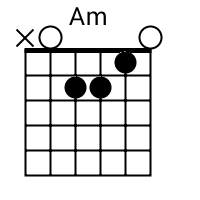
\includegraphics[scale=1.5]{../Akordy/am.png}
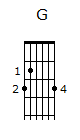
\includegraphics[scale=1.5]{../Akordy/g.png}
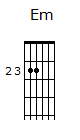
\includegraphics[scale=1.5]{../Akordy/em.png}
\end{figure}

\end{document}
